
% Template for a Computer Science Tripos Part II project dissertation
\documentclass[12pt,a4paper,twoside,openright]{report}
\usepackage[pdfborder={0 0 0}]{hyperref}    % turns references into hyperlinks
\usepackage[margin=20mm]{geometry}  % adjusts page layout
\usepackage[utf8]{inputenc}
\usepackage{graphicx}  % allows inclusion of PDF, PNG and JPG images
\usepackage{tikz}
\usepackage{subcaption}
\usepackage{minted}
\usepackage{color, colortbl}
\usepackage{diagbox}
\usepackage{verbatim}
\usepackage{caption}
\usepackage{datetime}
\usepackage{datenumber}
\usepackage{advdate}
\usepackage{titlesec}
\usepackage{pdfpages}
\usepackage[toc]{appendix}
\usepackage{subfiles}
\usepackage{amsmath}
\usepackage{amssymb}

\raggedbottom                           % try to avoid widows and orphans
\sloppy
\clubpenalty1000%
\widowpenalty1000%

\definecolor{Gray}{gray}{0.9}
      
\newmintinline[monospace]{text}{escapeinside=\#\#, mathescape, fontsize=\normalsize}
\newminted[pythonfigure]{python}{linenos, frame=single, framesep=2mm, autogobble, escapeinside=;;, mathescape}
\newminted[monospacefigure]{text}{linenos, frame=single, framesep=2mm, autogobble, escapeinside=;;, mathescape=true}

\renewcommand{\baselinestretch}{1.1}    % adjust line spacing to make
                                        % more readable

\begin{document}

\bibliographystyle{plain}


%%%%%%%%%%%%%%%%%%%%%%%%%%%%%%%%%%%%%%%%%%%%%%%%%%%%%%%%%%%%%%%%%%%%%%%%
% Title


\pagestyle{empty}

\rightline{\LARGE \textbf{Andrius Grabauskas}}

\vspace*{60mm}
\begin{center}
\Huge
\textbf{Measuring mutual information in Neural Networks} \\[5mm]
Computer Science Tripos -- Part II \\[5mm]
Robinson College \\[5mm]
\today  % today's date
\end{center}

%%%%%%%%%%%%%%%%%%%%%%%%%%%%%%%%%%%%%%%%%%%%%%%%%%%%%%%%%%%%%%%%%%%%%%%%%%%%%%
% Proforma, table of contents and list of figures

\pagestyle{plain}

\chapter*{Declaration}
\subfile{declaration}

\chapter*{Proforma}
\subfile{proforma}

\tableofcontents
\listoffigures

%%%%%%%%%%%%%%%%%%%%%%%%%%%%%%%%%%%%%%%%%%%%%%%%%%%%%%%%%%%%%%%%%%%%%%%
% now for the chapters

\pagestyle{headings}

\chapter{Introduction}
\subfile{introduction}

\chapter{Preparation}
\subfile{preparation}

\chapter{Implementation}
\subfile{implementation}


\chapter{Evaluation}
\subfile{evaluation}

\chapter{Conclusion}
\subfile{conclusion}

% TODO(ag939)

%%%%%%%%%%%%%%%%%%%%%%%%%%%%%%%%%%%%%%%%%%%%%%%%%%%%%%%%%%%%%%%%%%%%%
% the bibliography

\addcontentsline{toc}{chapter}{Bibliography}
\bibliography{refs}

%%%%%%%%%%%%%%%%%%%%%%%%%%%%%%%%%%%%%%%%%%%%%%%%%%%%%%%%%%%%%%%%%%%%%
% the appendices
\appendix

\chapter{Project Proposal}
\includepdf[pages={2,3,4,5}]{proposal.pdf}

\end{document}
